\chapter{Asking Texan Billionaires How They Got Rich!}

These notes follow a School of Hard Knocks interview episode, curated by LazyingArt LLC, and treat it as a lecture on commercial scale rather than as a mere sequence of street encounters. The host begins with spectacle, widens to a field of wealth in Texas, and then keeps asking the same deeper question in different forms: what hidden mechanism turns visible success into something reproducible? The mathematics here is light and schematic, but the lecture is full of quantitative anchors, allocation rules, and decision structures, and those are precisely what we preserve.

\section{Texas as a Wealth Field}

The lecture does not begin by explaining a method; it begins by proving access. We are shown, in compressed form, a sale at roughly eight hundred million dollars, companies doing more than a billion dollars a year, and visibly wealthy operators willing to stop and answer questions. Only after this compressed proof does the host tell us why the setting matters: Texas is not scenery but a field of concentrated wealth.

The opening numerical frame is simple enough to record.

\begin{align}
S_{\mathrm{sale}} &\approx \$800\times 10^{6},\\
R_{\mathrm{company}} &> \$850\times 10^{6},\\
R_{\mathrm{companies}} &> \$1\times 10^{9}\ \text{per year}.
\end{align}

These teaser values are then lifted into a geographic statement:

\begin{align}
N_{\mathrm{TX,billionaires}} &> 80,\\
\operatorname{rank}_{\mathrm{economy}}(\mathrm{Texas}) &= 8.
\end{align}

The point is not merely that Texas is rich. The point is that Austin is presented as a test site in which questions about money, industry, scale, and personal freedom can be asked almost experimentally. The lecture therefore begins in the register of field selection: first choose a place where large outcomes are dense, and only then ask what those outcomes mean.

\section{Action, Responsibility, and the First Wealth Machine}

The first long interview turns away from macro scale and toward the psychological threshold of entrepreneurship. The speaker has been in business for thirteen years, sells smoothies, and gives us a pair of revenue anchors:

\begin{equation}
R_{\mathrm{smoothie,last}} \approx \$23\times 10^{6},
\qquad
R_{\mathrm{smoothie,this}} \in [\$32,\$35]\times 10^{6}.
\end{equation}

That establishes that we are not listening to vague motivational talk. We are listening to someone whose moral vocabulary is tied to an actual business trajectory. The lecture then sharpens the question: is everybody built for entrepreneurship? The answer is deliberately blunt, and we record it in the leanest possible schematic form,

\begin{equation}
\mathcal{P}=\{\text{talkers},\ \text{doers}\}.
\end{equation}

This is not a theorem. It is an editorial compression of the interviewee's partition of human posture. Still, it is useful because the rest of the interview is really an attempt to explain what moves a person from one side of that partition to the other.

\subsection{Question \& Answer}

\paragraph{Question.} What actually separates wanting entrepreneurship from being built for it?

\paragraph{Answer.} In this lecture the answer is not an IQ measure, nor a credential, nor an industry secret. It is action under moral discipline. The speaker first separates talk from doing, and then immediately deepens that distinction into surrender, responsibility, work, saving, and investment. In other words, entrepreneurship is not introduced as a career label but as a sequence of transformations in conduct.

The internal logic of that sequence can be written schematically as
\begin{equation}
\text{surrender}
\to
\text{responsibility}
\to
\text{labor}
\to
\text{saving}
\to
\text{investing}.
\end{equation}

The lecture does not leave this in abstraction. The speaker supplies the before-state as well: years of victimhood, addiction, homelessness, and blame. What changes is not one tactic but the governing attribution of cause. Once fault is internalized, action becomes possible; once action becomes possible, money can be handled rather than merely desired.

We should note the financial advice in its minimal working form:
\begin{equation}
\text{income} - \text{spending} > 0
\quad\Longrightarrow\quad
\text{savings} > 0
\quad\Longrightarrow\quad
\text{investment capacity} > 0.
\end{equation}

This is elementary arithmetic, but it matters because the lecture embeds it inside biography. The accounting identity is not presented as textbook personal finance. It is presented as part of a reconstruction of agency.

The first doctrine block closes, strikingly, not on entrepreneurship but on family obligation: take care of one's mother, take care of family, do not use business ambition as an excuse for moral neglect. That ending matters. It prevents the lecture from reducing the entire question of wealth to a single metric.

\section{Mispriced Opportunity and the Geography of Capital}

The second major interview changes the scale of the argument. We move from personal reconstruction to capital allocation. The host asks for the best industry, and the answer arrives as a deliberate redefinition: not an industry in the narrow sense, but a geography, namely Africa.

The reasoning is comparative and asymmetrical. On the one hand, the speaker claims that
\begin{equation}
g_{\mathrm{Africa}}=\frac{9}{20},
\end{equation}
where \(g_{\mathrm{Africa}}\) is the reported share of the world's twenty fastest-growing economies in 2025. On the other hand, the capital share is said to be
\begin{equation}
\alpha_{\mathrm{Africa}} \approx 0.5\%.
\end{equation}

The lecture's claim is not that these two quantities can be compared as identical objects; rather, it is that their contrast is so extreme that it reveals neglect. Growth, demography, and technological leapfrogging are gathered together on one side; a tiny share of global private equity and venture capital is placed on the other.

\subsection{Question \& Answer}

\paragraph{Question.} How can a geography function like an industry-level opportunity?

\paragraph{Answer.} The lecture's answer is that investors do not only misprice firms; they misprice terrains. If one region combines rapid growth, a growing population, digital adoption, and low incoming capital, then the region itself can behave like an overlooked domain of entrepreneurial opportunity. The point is not taxonomic purity. The point is that capital follows categories, and categories can be wrong.

The transcript then moves into a partially garbled scaling discussion. We should not overconstruct that damaged segment. What survives clearly is an operating principle about labor and customers:
\begin{equation}
\text{care for employees}
\to
\text{better service to customers}
\to
\text{better ideas}
\to
\text{stronger business}.
\end{equation}

This is important because it prepares the host's next pivot. If the lecture begins with solitary-looking founders, it now starts undoing the myth of solitary success.

\section{The Hidden Team Behind the Visible Channel}

At this point the host turns the camera, briefly, back onto his own machine. He says the channel's growth did not happen because of him alone, and he names co-founders, editors, videographers, and strategists. Here the lecture becomes visually explicit: the selected frame shows the host on the street with a left-hand icon stack for people, editing, and camera work.

\begin{figure}
\centering

\includegraphics[width=0.78\textwidth]{lecture_43_figure_02.png}
\end{figure}

There is no literal board mathematics in this frame, but it does support a clean reconstruction of the role stack:
\begin{equation}
\mathcal{T}_{\mathrm{visible}}=\{\text{people/team},\ \text{editing},\ \text{camera}\},
\end{equation}
while the spoken list is slightly larger:
\begin{equation}
\mathcal{T}_{\mathrm{spoken}}
=
\{\text{co-founders},\ \text{editors},\ \text{videographers},\ \text{strategists}\}.
\end{equation}

The difference between these two sets matters. The first is supported directly by iconography; the second is supported by speech plus iconography. We therefore keep both, but we keep them distinct.

A cleaned organizational sketch can be drawn beside the screenshot:

\begin{figure}
\centering
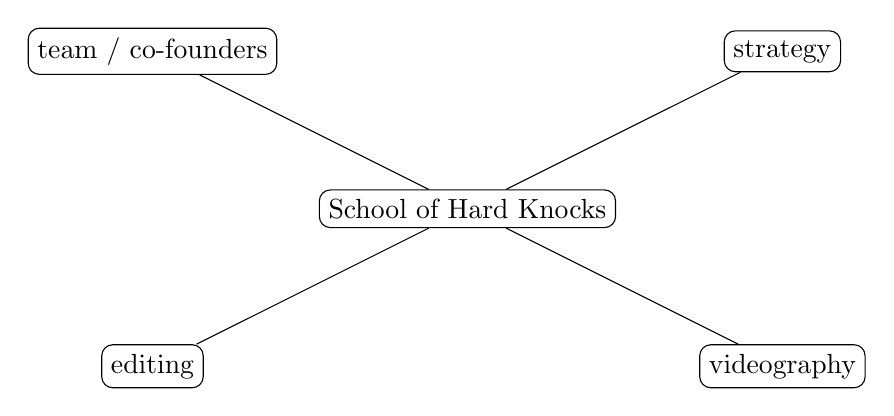
\begin{tikzpicture}
\node[draw, rounded corners] (s) at (0,0) {School of Hard Knocks};
\node[draw, rounded corners] (t) at (-4,2) {team / co-founders};
\node[draw, rounded corners] (e) at (-4,-2) {editing};
\node[draw, rounded corners] (v) at (4,-2) {videography};
\node[draw, rounded corners] (r) at (4,2) {strategy};
\draw (t) -- (s);
\draw (e) -- (s);
\draw (v) -- (s);
\draw (r) -- (s);
\end{tikzpicture}
\end{figure}

\subsection{Question \& Answer}

\paragraph{Question.} Why does the lecture interrupt itself to talk about the host's own team?

\paragraph{Answer.} Because otherwise the lecture would accidentally teach the wrong lesson. A string of interviews with wealthy individuals naturally centers faces. The team interlude corrects that optical illusion. It says, in effect, that output is organizational even when the narrative surface is personal. The later sponsor segment about hiring is therefore not a digression in theme. It extends the same proposition: building a dependable team is itself part of the business problem.

The host's own reported channel scale shifts slightly across the lecture, and we keep it approximate:
\begin{equation}
F_{\mathrm{host}} \approx 12\times 10^{6}
\quad\text{to}\quad
13\times 10^{6}.
\end{equation}

Again the point is not exact counting. The point is that even this scale is presented as distributed work.

\section{Health as Throughput, Not Ornament}

The Brian Johnson interview changes the register again. For a while the lecture stops asking where wealth is found or how teams are built, and asks what sort of organism is capable of carrying a large enterprise. The central claim is that health is not a decorative luxury placed beside entrepreneurship; it is an input into cognition and sustained performance.

The lecture's local chain is simple:
\begin{equation}
\text{sleep and health priority}
\to
\text{clearer thinking}
\to
\text{better entrepreneurial decisions}.
\end{equation}

This is then radicalized by a collection of self-reported quantities. Because the claims are speaker-attributed and unusually strong, we write them with caution:
\begin{align}
a_{\mathrm{chronological}} &= 47,\\
a_{\mathrm{biological}} &\approx 18,\\
N_{\mathrm{rejuvenation}} &\approx 5000,\\
T_{\mathrm{birthday}} &\approx 24\ \text{months}.
\end{align}

\begin{remark}
The age, competition, and slowed-aging claims in this section are self-reported. They are part of the lecture's argumentative structure, but they are not to be silently converted into neutral scientific fact.
\end{remark}

\subsection{Question \& Answer}

\paragraph{Question.} Can health be a higher-yield business input than more grind?

\paragraph{Answer.} In this lecture, yes. The host asks for business advice and receives a reframing: the relevant bottleneck is often not effort but throughput. If grind lowers clarity, then more grind can become self-defeating. Health, then, is treated as a productivity multiplier rather than a reward one purchases after success.

The interview then pushes further into speculative longevity claims and environmental toxicity. We should preserve the progression, because it is part of the lecture's rhythm. What begins as a practical correction---sleep, health, mental clarity---widens into a frontier ambition: why think only in decades, if technology and biology might stretch the horizon? The notes should preserve that widening, while also preserving its attributed status.

\section{The 90/10 Rule and the Trust Geometry of Enterprise Sales}

The final major interview provides the lecture's sharpest piece of explicit arithmetic. We are told to spend about ninety percent of our time on the present job and ten percent on the career. The value of this rule lies in its contrast with two neighboring errors.

We can write the three cases as
\begin{equation}
(t_{\mathrm{job}},t_{\mathrm{career}})
\in
\{(1.0,0.0),\ (0.9,0.1),\ (0.8,0.2)\}.
\end{equation}

The lecture's reasoning is then a worked comparison:
\begin{enumerate}
\item If \((t_{\mathrm{job}},t_{\mathrm{career}})=(1.0,0.0)\), one may perform extremely well locally, but one does not build enough outward visibility, connection, or next-step awareness.
\item If \((t_{\mathrm{job}},t_{\mathrm{career}})=(0.8,0.2)\), one spends too much time circling the future and not enough time earning the present role.
\item Therefore the lecture selects
\begin{equation}
t_{\mathrm{job}} \approx 0.9,
\qquad
t_{\mathrm{career}} \approx 0.1,
\end{equation}
as the practical balance.
\end{enumerate}

\subsection{Question \& Answer}

\paragraph{Question.} Why is \(90/10\) better than both total job-focus and excessive career-optimization?

\paragraph{Answer.} Because the lecture treats careers as path-dependent. Present excellence without outward movement traps the worker inside the current role, while outward movement without present excellence destroys the quality that makes advancement deserved. The \(90/10\) rule is therefore not a theorem of optimization; it is a disciplined compromise between performance and trajectory.

The interview then turns from career arithmetic to enterprise sales. The company sells to large businesses, and that alone changes the geometry of the sale:
\begin{align}
T_{\mathrm{sales}} &\ge 1\ \text{year},\\
n_{\mathrm{stakeholders}} &\approx 50.
\end{align}

This is not one conversation with one buyer. It is a chain of proof, reference, and institutional confidence. The lecture gives the cleanest schematic of the whole episode here:
\begin{equation}
\text{proof of concept}+\text{references}+\text{partner trust}\to\text{purchase}.
\end{equation}

We can unpack that in order:
\begin{enumerate}
\item A large firm must first see the technology work.
\item It must then see that comparable firms trust it.
\item Only after that does it conclude that the seller is the right partner.
\item Only then does money move.
\end{enumerate}

The scale claim attached to this business is itself substantial:
\begin{equation}
\frac{1}{2}\text{ of the Fortune 500 are said to be customers.}
\end{equation}

The lecture closes not with sales tactics alone, but with a broader triad: find the right team, attack a large enough problem, and do not let identity collapse entirely into business status. That last move is essential. It reconnects the final founder to the lecture's earlier moral vocabulary. Faith, family, and worth outside the firm are not treated as anti-business. They are treated as the conditions under which business success does not hollow out the person who attains it.

\section{Summary}

The lecture proceeds by repeated enlargements and corrections. First it shows wealth, then it asks what structure produced it. First it isolates founders, then it restores teams. First it speaks of revenue and exits, then it asks about discipline, health, and identity. The notes therefore preserve not a single doctrine but a sequence of linked propositions: Texas as a field of scale, action as the first entrepreneurial partition, responsibility as the first wealth machine, Africa as mispriced opportunity, team as hidden production, health as throughput, and \(90/10\) as a rule for balancing present excellence with future movement. The final lesson is that scale is neither purely financial nor purely personal. It is a compound of arithmetic, organization, and character.